\begin{chapter}{Dynamisches Programmieren}
\begin{section}{Dominating Set}
  \begin{definition}
   Sei ein Graph \(G = (V,E)\) gegeben. Wir nennen eine Menge \(D \subseteq V\) \defNotion{dominierend} für $G$, falls jeder Knoten $v \in V$ entweder in $D$ liegt, oder adjazent zu einem Knoten aus $D$ ist.
  \end{definition}
  \paragraph{Problem Minimum Dominating Set (MDS).} Eingabe ist ein Graph $G=(V,E)$, gesucht ist eine Dominierende Menge $D$ für $G$ mit minimaler Kardinalität $\gamma(G)$.

  Ein brute-force-Algorithmus für das kleinste dominating set läuft in \(O^*(2^n)\) durch Ausprobieren aller Teilmengen von \(V\). Zur Verbesserung dieser Laufzeit betrachten wir nicht erweiterbare unabhängige Mengen (UM) und verwenden dynamische Progammierung. 
  
  \begin{lemma}
   Eine UM lässt sich effizient berechnen.
  \end{lemma}
  \begin{proof}
  Der folgende Algorithmus hat Laufzeit $O(n+m)$ und löst das gegebene Problem. 
  
  \begin{algorithm}[H]
    \caption{Algorithmus zum Bestimmen einer nicht-erweiterbaren Unabhängingen Menge}

    \KwName{neUM} \\
    \KwData{Graph $G$}
    \KwResult{nicht-erweiterbare UM}
    \uIf{$V=\emptyset$}{
      \Return $\emptyset$
    }
    Wähle $v \in V$ mit höchstem Grad\\
    \Return $v + $ neUM($G-N[v]$)
  \end{algorithm}
  \end{proof}
  
  \begin{lemma}
   Jede nicht erweiterbare UM $I$ eines Graphen $G$ ist dominierend für $G$.
  \end{lemma}
  \begin{proof}
   Angenommen, dass nicht, dann gäbe es ein $v\in V-I$, dass nicht adjazent zu Knoten aus $I$ ist. Dann wäre $I + v$ eine unabhängige Menge, Widerspruch zur Nichterweiterbarkeit.
  \end{proof}

  \paragraph{Idee.} Zunächst bestimmen wir ein nicht-erweiterbare UM \(I\) für $G$. Dann verfahren wir wie folgt:
  \begin{enumerate}[i)]
   \item Falls dieses ``genügend klein'' ($|I| \leq\alpha \cdot n$) ist, können wir alle Knotenmengen \(D \subseteq V\) mit \(|D| \leq |I|\) ausprobieren. 
   \item Falls \(I\) ``groß'' ($|I| > \alpha \cdot n$) ist, wenden wir das folgende Verfahren an, dass sich aus der Struktur von $G$ ergibt.
  \end{enumerate}

  \begin{lemma}
  \label{domSet}
    Sei \(G\) ein Graph und \(I\) eine nicht-erweiterbare UM für $G$. Dann lässt sich eine kleinste dominierende Menge für $G$ in \(O^*(2^{n-|I|})\) ermitteln.
  \end{lemma}

  %Beweis fehlt.

  \begin{proof}
    Wir definieren uns eine Menge $J \isDefinedBy V -I$. Anstatt alle $2^n$ Teilmengen $D\subseteq V$ zu betrachten, probieren wir ``nur'' die $2^{|J|} = 2^{n-|I|}$ vielen Projektionen \(J_D \isDefinedBy D \cap J\) von allen möglichen $D\subseteq V$ in $J$. Wir bestimmen eine dominierende Menge $D$ mit den Eigenschaften: 
    \begin{itemize}
     \item $J_D = J \cap D$ und 
     \item $|D| = \min \{|D'|: D' \text{ dominierende Menge}, J_D = J \cap D'\}$.
    \end{itemize}
    Für diese Menge gilt dann $D = J_D \cup I_D$, wobei \(I_D \isDefinedBy I \setminus N(J_D)\). Dann folgt daraus 
    \[\gamma(G) = \min_{J_D \subseteq J} |D|\text{.}\]
    Es bleibt die Frage, wie man von $J_D$ auf $D$ kommt. Es gilt, dass $I_D \subseteq D$, da $I_D$ von keinem Knoten aus $I - I_D$ und $J$ dominiert werden kann. Die einzigen von $I_D \cup J_D$ noch nicht dominierten Knoten sind die Knoten:
    \[J_X \isDefinedBy J - (N[J_D]\cup N(I_D))\text{.}\]
    Um $D$ zu ermitteln, müssen wir daher ``nur'' die kleine Menge $D_{J_X} \subseteq I - I_X$ finden, die $J_X$ dominiert. Dann ist $D= J_D \cup I_D \cup D_{J_X}$.

    Der naive Ansatz wäre, für jedes $J_X$ das entsprechende $D_{J_X}$ seperat zu bestimmen. Dies ist jedoch zu langsam. Cleverer bestimmt man simultan für jedes $X \subseteq J$ das kleinste $D_X \subseteq I$, dass $X$ dominiert. Dazu betrachten wir folgendes dynamisches Programm:
    
    \underline{Dynamisches Programm:}\\
    Sei $I = \{v_1,\dots,v_k\}$. Dann sei $D_{X,i}$ die kleinste Teilmenge von $\{v_1,\dots,v_k\}$, die $X$ dominiert. $\Rightarrow$ $D_X = D_{X,R}$.\\
    \begin{itemize}
     \item $i = 0$:\\
      $D_{X,0} = \begin{cases}
		  \emptyset & \text{ falls } X = \emptyset\\
		  \{v_1,\dots,v_k\} & \text{ falls } X \neq \emptyset
               \end{cases}$
     \item $i \geq 1$:\\
     $D_{X,i} = $ die kleinere der Mengen $D_{X,i-1}$ und $D_{X-N(v_i),i-1} \cup \{v_i\}$
    \end{itemize}
    Laufeit des dyn. Programms: $O(2^{|J|\cdot n^2}) = O^*(2^{|J|})$
    
    \underline{Gesamte Laufzeit des Algorithmus:}\\
    \begin{itemize}
     \item dyn. Programm: $O^*(2^{|J|})$
     \item ermittle für jedes der $2^{|J|}$-vielen $J_D \subseteq J$ die Menge $I_D,J_X,D_{J_X}$, wobei sich die dominierende Menge durch $D= I_D \cup J_D \cup D_{J_X}$ ergibt. $\Rightarrow O^*(2^{|J|})$
    \end{itemize}
    $\Rightarrow O^*(2^{|J|})= O^*(2^{n-|I|})$
  \end{proof}  
  
  \begin{lemma}[Hilfslemma]
    Sei $\alpha \leq \frac{1}{2}$, dann ist
    \[\sum_{k=0}^{\alpha n} \binom{n}{k} = O^*(2^{h(\alpha) \cdot n})\text{,}\]
    wobei $h(\alpha) = -\alpha\log_2 \alpha - (1-\alpha) \log_2 (1-\alpha)$.
      \begin{figure}[H]
	\centering
	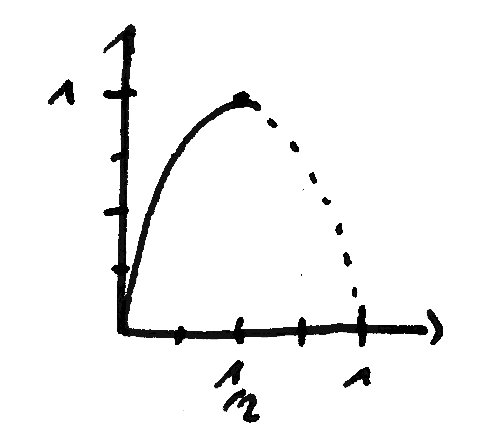
\includegraphics[width=.25\textwidth]{./Bilder/b01.jpg}
	% b01.jpg: 495x434 pixel, 72dpi, 17.46x15.31 cm, bb=0 0 495 434
	\caption{Graph des Binomialkoeffizienten}
      \end{figure}
  \end{lemma}
  \begin{proof}
    Es ist \( \sum_{i=0}^{\alpha n} \leq n \binom{n}{\alpha n} = O^*( \binom{n}{\alpha n} ) \), denn die Binomialkoeffizienten \( \binom{a}{b} \) steigen für \(b \leq n/2\) monoton an. Per Definition gilt 
    \[ \binom{n}{k} = \frac{n!}{k! (n-k)!}. \]
    Die Fakultät kann abgeschätzt werden durch \( \sqrt{2 \pi n} (n/e)^n \leq n! \leq 2 \sqrt{2 \pi n} (n/e)^n \), also ist \(n!\) proportional zu \((n/e)^n\). Daraus folgt, dass 
    \begin{eqnarray*}
      \binom{n}{\alpha n} &=& O^* \left( \frac{(n/e)^n}{(\alpha n/e)^{\alpha n} ( (1-\alpha)n/e)^{(1-\alpha) n}} \right) = O^* \left( \alpha^{-\alpha n} (1-\alpha)^{-(1-\alpha)n} \right) \\
      &=& O^* \left( 2^{-\alpha \log_2 \alpha n} \cdot 2^{-(1 - \alpha) \log_2(1-\alpha)n} \right),
    \end{eqnarray*}
    woraus die Behauptung folgt.
  \end{proof}

  \begin{theorem}
    Eine kleinste dominierende Menge lässt sich in \(O(1{,}7088^n)\) ermitteln.
  \end{theorem}
  \begin{proof}
    Zunächst bestimmen wir eine nicht-erweiterbare unabhänge Menge \(I\). 
    Falls \(|I| \leq \alpha n\), testen wir in \(O^*(2^{h(\alpha) n})\) alle Teilmengen \(D \subseteq V\) mit \(|D| \leq |I|\).
    Falls \(|I| > \alpha n\), wende Lemma \ref{domSet} an und berechne kleinste dominierende Menge in \(O^*(2^{(1-\alpha)n})\). % Satz in dem O*(2^(n-|I|)) bewiesen wurde
    
    \begin{figure}[h]
      \centering
      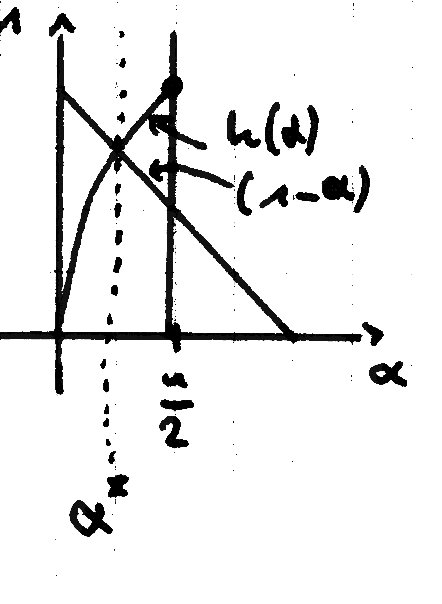
\includegraphics[width=.25\textwidth]{./Bilder/b02.jpg}
      % b02.jpg: 442x604 pixel, 72dpi, 15.59x21.31 cm, bb=0 0 442 604
      \caption{Bestimmung von \(\alpha^*\) als Maximum der zwei möglichen Funktionen}
    \end{figure}
    
    Aus der Skizze ergibt sich die Laufzeit als das Maximum der beiden dargestellten Funktionen bei \(\alpha^* \leq 0,22711\) bzw. \(O(2^{0,7729n}) = O(1,7088^n)\).
  \end{proof}
  
  Der schnellste derzeit bekannte Algorithmus für dieses Problem benötigt ca. \(O(1,5^n)\) und stammt aus 2010.
\end{section}
\end{chapter}